\documentclass[a4paper,12pt]{article}  % Klasa dokumentu
\usepackage[polish]{babel}              % Język dokumentu
\usepackage{amsmath, amssymb}           % Pakiety matematyczne
\usepackage{graphicx}                   % Do wstawiania grafiki
\usepackage{hyperref}                   % Linki w dokumencie
\usepackage{geometry}                   % Ustawienia marginesów
\usepackage{float}
\usepackage[T1]{fontenc}
\usepackage{subfigure}
\geometry{margin=1in}                   % Definicja marginesów
\usepackage{array}
\usepackage{caption}
\usepackage{subcaption}

% Tytuł i autor
\title{Obrazy kanałowe i wskaźniki spektralne}
\author{Adrian Fabisiewicz}
\date{\today}

\begin{document}

\maketitle  % Tworzenie tytułu

\section{Cel zadania}
Celem zadania było zbadanie:
\begin{itemize}
    \item jak różne klasy obiektów odwzorowują się na obrazach w spektrum widzialnym (RGB) oraz w bliskiej podczerwieni (IR) 
    \item w jaki sposób kompozycje barwne mogą ułatwić interpretację klas obiektów na zdjęciach
    \item roli wskaźników spektralnych w interpretacji obrazów
\end{itemize}

\section{Dane do zadania}
Danymi do zadania były zdjęcia zarejestrowane w zakresie RGB oraz CIR z lat 2015 i 2023 oraz stworzona na ich podstawie poligonowa warstwa wektorowa, zawierająca budynki.

\newpage
\section{Realizacja}
\subsection{Przedstawienie obiektów w poszczególnych kanałach spektralnych}

\subsubsection{Budynek 1.}

\begin{figure}[H]
    \centering
    \begin{minipage}{0.24\textwidth}
        \centering
        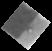
\includegraphics[width=\linewidth]{spektralne/nir_budynek7.png}
        \caption*{NIR}
    \end{minipage}
    \begin{minipage}{0.24\textwidth}
        \centering
        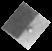
\includegraphics[width=\linewidth]{spektralne/red_budynek7.png}
        \caption*{RED}
    \end{minipage}
    \begin{minipage}{0.24\textwidth}
        \centering
        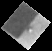
\includegraphics[width=\linewidth]{spektralne/green_budynek7.png}
        \caption*{GREEN}
    \end{minipage}
    \begin{minipage}{0.24\textwidth}
        \centering
        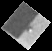
\includegraphics[width=\linewidth]{spektralne/blue_budynek7.png}
        \caption*{BLUE}
    \end{minipage}
\end{figure}

\subsubsection{Budynek 2.}
\begin{figure}[H]
    \centering
    \begin{minipage}{0.24\textwidth}
        \centering
        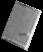
\includegraphics[width=\linewidth]{spektralne/nir_budynek0.png}
        \caption*{NIR}
    \end{minipage}
    \begin{minipage}{0.24\textwidth}
        \centering
        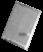
\includegraphics[width=\linewidth]{spektralne/red_budynek0.png}
        \caption*{RED}
    \end{minipage}
    \begin{minipage}{0.24\textwidth}
        \centering
        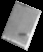
\includegraphics[width=\linewidth]{spektralne/green_budynek0.png}
        \caption*{GREEN}
    \end{minipage}
    \begin{minipage}{0.24\textwidth}
        \centering
        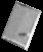
\includegraphics[width=\linewidth]{spektralne/blue_budynek0.png}
        \caption*{BLUE}
    \end{minipage}
\end{figure}

\subsubsection{Budynek 3.}

\begin{figure}[H]
    \centering
    \begin{minipage}{0.24\textwidth}
        \centering
        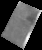
\includegraphics[width=\linewidth]{spektralne/nir_budynek3.png}
        \caption*{NIR}
    \end{minipage}
    \begin{minipage}{0.24\textwidth}
        \centering
        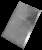
\includegraphics[width=\linewidth]{spektralne/red_budynek3.png}
        \caption*{RED}
    \end{minipage}
    \begin{minipage}{0.24\textwidth}
        \centering
        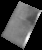
\includegraphics[width=\linewidth]{spektralne/green_budynek3.png}
        \caption*{GREEN}
    \end{minipage}
    \begin{minipage}{0.24\textwidth}
        \centering
        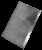
\includegraphics[width=\linewidth]{spektralne/blue_budynek3.png}
        \caption*{BLUE}
    \end{minipage}
\end{figure}

\newpage
\subsection{Zestawienie wybranych statystyk numerycznych w poszczególnych kanałach obrazu.}

\begin{table}[h!]
\centering
\begin{tabular}{|c|c|c|c|}
\hline
\multicolumn{4}{|c|}{\textbf{Budynek 1.}} \\ \hline
\textbf{} & \textbf{min} & \textbf{max} & \textbf{mean} \\ \hline
\textbf{NIR} & 48 & 157 & 77\\ \hline
\textbf{RED} & 40 & 131 & 70\\ \hline
\textbf{GREEN} & 43 & 134 & 71\\ \hline
\textbf{BLUE} & 37 & 120 & 65\\ \hline
\end{tabular}
\end{table}

\begin{table}[h!]
\centering
\begin{tabular}{|c|c|c|c|}
\hline
\multicolumn{4}{|c|}{\textbf{Budynek 2.}} \\ \hline
\textbf{} & \textbf{min} & \textbf{max} & \textbf{mean} \\ \hline
\textbf{NIR} & 39 & 187 & 101\\ \hline
\textbf{RED} & 47 & 203 & 127\\ \hline
\textbf{GREEN} & 60 & 217 & 133\\ \hline
\textbf{BLUE} & 43 & 205 & 128\\ \hline
\end{tabular}
\end{table}

\begin{table}[h!]
\centering
\begin{tabular}{|c|c|c|c|}
\hline
\multicolumn{4}{|c|}{\textbf{Budynek 3.}} \\ \hline
\textbf{} & \textbf{min} & \textbf{max} & \textbf{mean} \\ \hline
\textbf{NIR} & 59 & 178 & 90\\ \hline
\textbf{RED} & 60 & 189 & 99\\ \hline
\textbf{GREEN} & 55 & 193 & 97\\ \hline
\textbf{BLUE} & 44 & 191 & 92\\ \hline
\end{tabular}
\end{table}

\newpage
\subsection{Porównanie wyglądu obiektów na kompozycjach barwnych RGB, IrGB oraz dwóch innych wybranych kompozycjach}

\subsubsection{Budynek 1.}
\begin{figure}[H]
    \centering
    \begin{minipage}{0.24\textwidth}
        \centering
        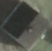
\includegraphics[width=\linewidth]{spektralne/rgb_budynek7.png}
        \caption*{RGB}
    \end{minipage}
    \begin{minipage}{0.24\textwidth}
        \centering
        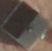
\includegraphics[width=\linewidth]{spektralne/irgb_budynek7.png}
        \caption*{IrGB}
    \end{minipage}
    \begin{minipage}{0.24\textwidth}
        \centering
        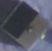
\includegraphics[width=\linewidth]{spektralne/rgir_budynek7.png}
        \caption*{RGIr}
    \end{minipage}
    \begin{minipage}{0.24\textwidth}
        \centering
        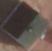
\includegraphics[width=\linewidth]{spektralne/irrb_budynek7.png}
        \caption*{IrRB}
    \end{minipage}
\end{figure}

\subsubsection{Budynek 2.}
\begin{figure}[H]
    \centering
    \begin{minipage}{0.24\textwidth}
        \centering
        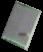
\includegraphics[width=\linewidth]{spektralne/rgb_budynek0.png}
        \caption*{RGB}
    \end{minipage}
    \begin{minipage}{0.24\textwidth}
        \centering
        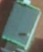
\includegraphics[width=\linewidth]{spektralne/irgb_budynek0.png}
        \caption*{IrGB}
    \end{minipage}
    \begin{minipage}{0.24\textwidth}
        \centering
        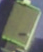
\includegraphics[width=\linewidth]{spektralne/rgir_budynek0.png}
        \caption*{RGIr}
    \end{minipage}
    \begin{minipage}{0.24\textwidth}
        \centering
        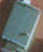
\includegraphics[width=\linewidth]{spektralne/irrb_budynek0.png}
        \caption*{IrRB}
    \end{minipage}
\end{figure}

\subsubsection{Budynek 3.}
\begin{figure}[H]
    \centering
    \begin{minipage}{0.24\textwidth}
        \centering
        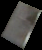
\includegraphics[width=\linewidth]{spektralne/rgb_budynek3.png}
        \caption*{RGB}
    \end{minipage}
    \begin{minipage}{0.24\textwidth}
        \centering
        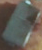
\includegraphics[width=\linewidth]{spektralne/irgb_budynek3.png}
        \caption*{IrGB}
    \end{minipage}
    \begin{minipage}{0.24\textwidth}
        \centering
        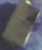
\includegraphics[width=\linewidth]{spektralne/rgir_budynek3.png}
        \caption*{RGIr}
    \end{minipage}
    \begin{minipage}{0.24\textwidth}
        \centering
        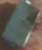
\includegraphics[width=\linewidth]{spektralne/irrb_budynek3.png}
        \caption*{IrRB}
    \end{minipage}
\end{figure}

\newpage
\subsection{Porównanie wyglądu obiektów na wskaźniku spektralnym NDVI oraz jednym innym wybranym wskaźniku}
\subsubsection{Budynek 1.}
\begin{figure}[H]
    \centering
    \begin{minipage}{0.45\textwidth}
        \centering
        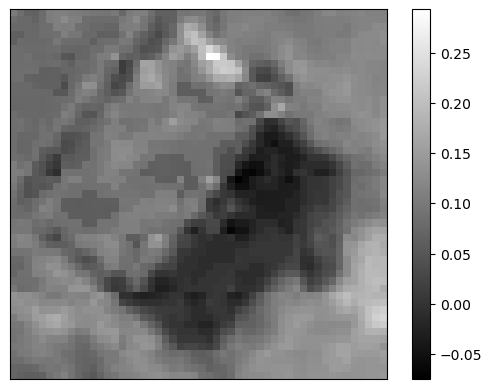
\includegraphics[width=\linewidth]{spektralne/ndvi_budynek7_2015.png}
        \caption*{NDVI 2015}
    \end{minipage}
    \begin{minipage}{0.45\textwidth}
        \centering
        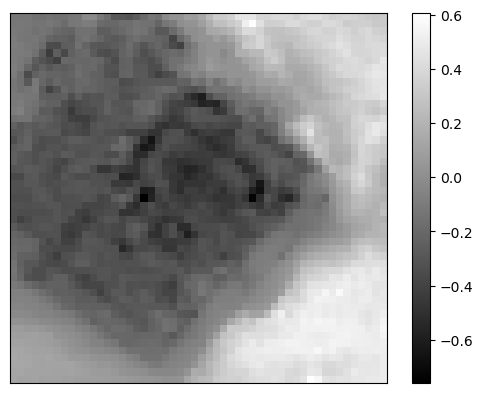
\includegraphics[width=\linewidth]{spektralne/ndvi_budynek7_2023.png}
        \caption*{NDVI 2023}
    \end{minipage}
\end{figure}

\begin{figure}[H]
    \centering
    \begin{minipage}{0.45\textwidth}
        \centering
        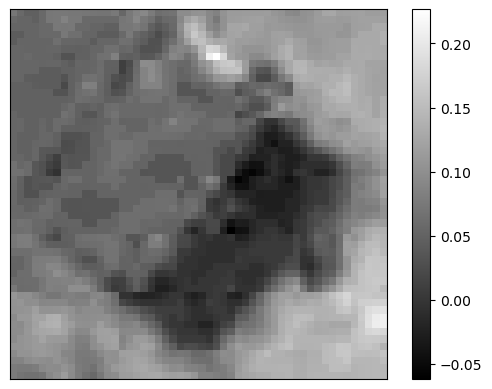
\includegraphics[width=\linewidth]{spektralne/msavi_budynek7_2015.png}
        \caption*{MSAVI 2015}
    \end{minipage}
    \begin{minipage}{0.45\textwidth}
        \centering
        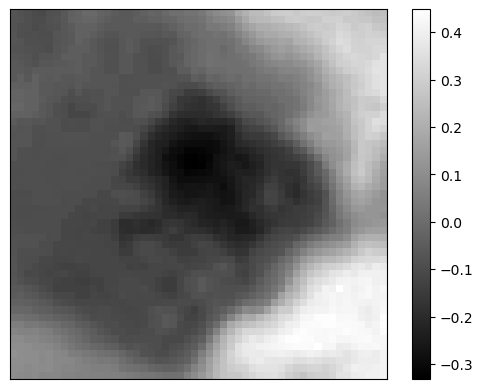
\includegraphics[width=\linewidth]{spektralne/msavi_budynek7_2023.png}
        \caption*{MSAVI 2023}
    \end{minipage}
\end{figure}

\newpage
\subsubsection{Budynek 2.}

\begin{figure}[H]
    \centering
    \begin{minipage}{0.45\textwidth}
        \centering
        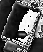
\includegraphics[width=\linewidth]{spektralne/ndvi_budynek0_2015.png}
        \caption*{NDVI 2015}
    \end{minipage}
    \begin{minipage}{0.45\textwidth}
        \centering
        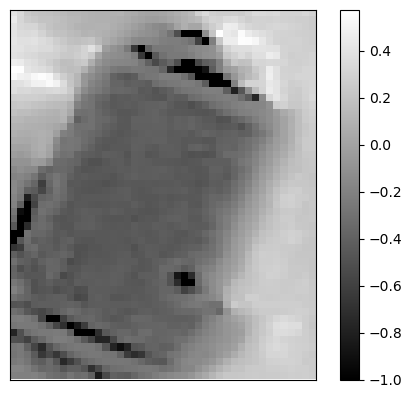
\includegraphics[width=\linewidth]{spektralne/ndvi_budynek0_2023.png}
        \caption*{NDVI 2023}
    \end{minipage}
\end{figure}

\begin{figure}[H]
    \centering
    \begin{minipage}{0.45\textwidth}
        \centering
        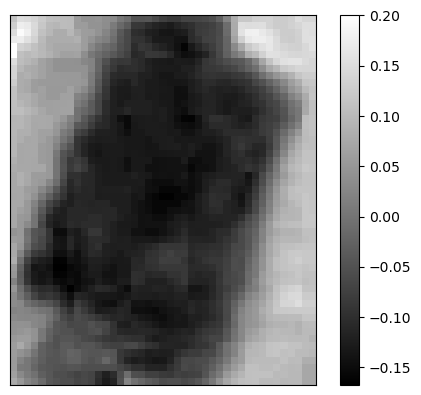
\includegraphics[width=\linewidth]{spektralne/msavi_budynek0_2015.png}
        \caption*{MSAVI 2015}
    \end{minipage}
    \begin{minipage}{0.45\textwidth}
        \centering
        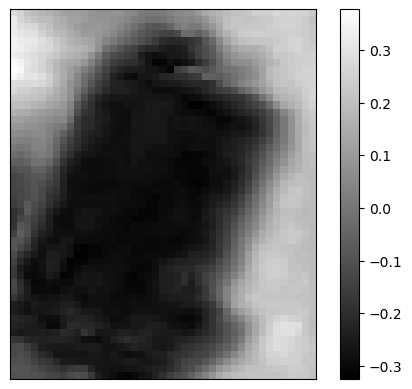
\includegraphics[width=\linewidth]{spektralne/msavi_budynek0_2023.png}
        \caption*{MSAVI 2023}
    \end{minipage}
\end{figure}

\subsubsection{Budynek 3.}

\begin{figure}[H]
    \centering
    \begin{minipage}{0.45\textwidth}
        \centering
        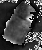
\includegraphics[width=\linewidth]{spektralne/ndvi_budynek3_2015.png}
        \caption*{NDVI 2015}
    \end{minipage}
    \begin{minipage}{0.45\textwidth}
        \centering
        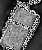
\includegraphics[width=\linewidth]{spektralne/ndvi_budynek3_2023.png}
        \caption*{NDVI 2023}
    \end{minipage}
\end{figure}

\begin{figure}[H]
    \centering
    \begin{minipage}{0.45\textwidth}
        \centering
        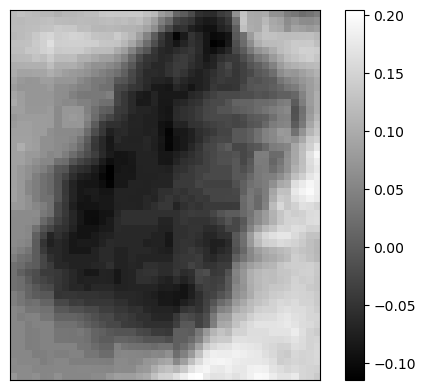
\includegraphics[width=\linewidth]{spektralne/msavi_budynek3_2015.png}
        \caption*{MSAVI 2015}
    \end{minipage}
    \begin{minipage}{0.45\textwidth}
        \centering
        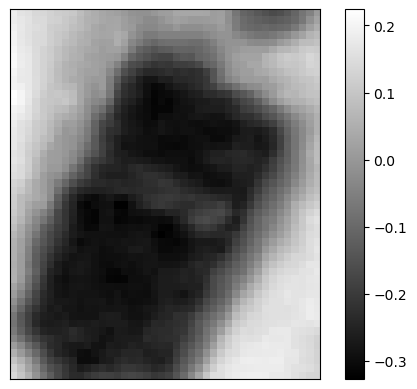
\includegraphics[width=\linewidth]{spektralne/msavi_budynek3_2023.png}
        \caption*{MSAVI 2023}
    \end{minipage}
\end{figure}

\newpage
\subsection{Zestawienie dla wskaźników spektralnych wartości statystycznych wyznaczonych na danych z 2015 oraz 2023 roku}

\begin{table}[h!]
    \centering
    \begin{tabular}{|c|c|c|c|}
    \hline
    \multicolumn{4}{|c|}{\textbf{Budynek 1.}} \\ \hline
    \textbf{} & \textbf{min} & \textbf{max} & \textbf{średnia} \\ \hline
    \textbf{NDVI 2015} & -0.08 & 0.29 & 0.03\\ \hline
    \textbf{NDVI 2023} & -0.76 & 0.45 & -0.11\\ \hline
    \textbf{MSAVI 2015} & -0.06 & 0.23 & 0.02\\ \hline
    \textbf{MSAVI 2023} & -0.33 & 0.33 & -0.05\\ \hline
    \end{tabular}
\end{table}

\begin{table}[h!]
    \centering
    \begin{tabular}{|c|c|c|c|}
    \hline
    \multicolumn{4}{|c|}{\textbf{Budynek 2.}} \\ \hline
    \textbf{} & \textbf{min} & \textbf{max} & \textbf{średnia} \\ \hline
    \textbf{NDVI 2015} & -0.24 & 0.07 & -0.06\\ \hline
    \textbf{NDVI 2023} & -1.0 & 0.47 & -0.18\\ \hline
    \textbf{MSAVI 2015} & -0.17 & 0.08 & -0.06\\ \hline
    \textbf{MSAVI 2023} & -0.33 & 0.24 & -0.12\\ \hline
    \end{tabular}
\end{table}

\begin{table}[h!]
    \centering
    \begin{tabular}{|c|c|c|c|}
    \hline
    \multicolumn{4}{|c|}{\textbf{Budynek 3.}} \\ \hline
    \textbf{} & \textbf{min} & \textbf{max} & \textbf{średnia} \\ \hline
    \textbf{NDVI 2015} & -0.14 & 0.21 & -0.02\\ \hline
    \textbf{NDVI 2023} & -1.0 & 0.16 & -0.19\\ \hline
    \textbf{MSAVI 2015} & -0.11 & 0.18 & -0.02\\ \hline
    \textbf{MSAVI 2023} & -0.33 & 0.10 & -0.11\\ \hline
    \end{tabular}
\end{table}

\newpage
\section{Komentarz}

W kanałach spektralnych R, G i B każdy obiekt wygląda bardzo podobnie. W kanale NIR obiekty są lekko ciemniejsze. Dla budynku 1. wartości dla wszystkich kanałów są najniższe, przyjmując maksimum 157 dla NIR. Dla budynku 2. średnie wartości są najwyższe i mają wartość ok. 130 dla kanałów R, G i B, gdzie średnia dla kanału NIR wynosi 101. Najmniejsza wartość to 37 dla kanału B dla budynku 1., a największa - 217 dla kanału G dla budynku 2.

Z wybranych 4 kompozycji barwnych na zdjęciach RGB wybrane budynki wydają się najtrudniej rozróżnialne. Mają barwy podobne do otoczenia i zlewają się z nim. Na pozostałych kompozycjach, tj. IrGB, RGIr oraz IrRB budynki na podobnym poziomie bardziej kontrastrują z otoczeniem, przyjmując na przykład barwę żółtą przy fioletowej barwie otoczenia lub barwę niebieską przy czerwonej barwie otoczenia. Łatwość interpretacji zależy od kanałów, z jakich utworzono kompozycję barwną. Jeżeli wybrane promieniowanie jest w różny sposób odbijane przez wykrywane przez nas obiekty oraz ich otoczenie, wtedy obiekty będą łatwiejsze do rozróżnienia. W przypadku wybranych przeze mnie kompozycji na łatwość wykrycia obiektów wpływa obecność kanału Ir.

W przypadku budynku 2. i 3. obydwa wskaźniki spektralne umożliwiają lepszą interpretację obiektów. Różnice między obiektami i ich otoczeniem są równie dobrze uwydatnione. Budynek 1. bardziej zlewa się z otoczeniem i byłoby trudniej określić jego dokładne granice.

Wartości NDVI w 2023 roku są średnio niższe niż w 2015: dla obiektu 1. nastąpił spadek średniej wartości NDVI z 0.03 do -0.11, dla obiektu 2.: z -0.06 do -0.18, a dla obiektu 3.: z -0.02 do -0.19. Podobne spadki nastąpiły dla MSAVI: z 0.02 do -0.05 dla obiektu 1., z -0.06 do -0.12 dla obiektu 2. oraz z -0.02 do -0.11 dla obiektu 3. Dla danych z 2023 roku występuje większa rozpiętość wartości dla obu wskaźników.

\end{document}